\documentclass{beamer}
\setbeamercovered{highly dynamic}
\usepackage[utf8]{inputenc}
\usepackage[T1]{fontenc}
\usepackage{lmodern}
\usetheme{Madrid}
\usepackage{tikz}
\usetikzlibrary{automata, positioning, arrows}
\usepackage{graphicx, animate}
\usepackage{movie15}
\graphicspath{ {./imagens/} }

\AtBeginSection[]{
	\begin{frame}
		\vfill
		\centering
		\begin{beamercolorbox}[sep=8pt,center,shadow=true,rounded=true]{title}
			\usebeamerfont{title}\insertsectionhead\par%
		\end{beamercolorbox}
		\vfill
	\end{frame}
}

\AtBeginSubsection[]{
	\begin{frame}
		\vfill
		\centering
		\begin{beamercolorbox}[sep=8pt,center,shadow=true,rounded=true]{title}
			\usebeamerfont{title}\insertsubsectionhead\par%
		\end{beamercolorbox}
		\vfill
	\end{frame}
}


\tikzset{
	node distance=3cm, % specifies the minimum distance between two nodes. Change if necessary.
	every state/.style={thick, fill=gray!10}, % sets the properties for each ’state’ node
	initial text=$ $, % sets the text that appears on the start arrow
}


\title{Metodologia de Pesquisa}
\subtitle{Simulação}
\author{Ricardo Rosal}
\begin{document}
	\begin{frame}[plain]
	\maketitle
	\end{frame}	
	\begin{frame}
		\tableofcontents
	\end{frame}
	\section{Simulação como método de pesquisa}
	\begin{frame}{Simulação como método de pesquisa}
		\begin{itemize}[<+->]
			\item O principal valor da simulação como método de pesquisa é a flexibilidade dada ao pesquisar de "abraçar" a complexidade do sistema e do modelo em um estudo e fazer perguntas do tipo \textbf{"e se?"} ao ínves de perguntas como \textbf{"o que aconteceu? como? e por que?"}.
			\item outros métodos de pesquisa, em contra-partida, requer que seja \textbf{estabelescida algumas preposições sobre causalidade do fenômeno estudado}, já a simulação nos permite, desde a dinâmica estabelescida do modelo, \textbf{"criar/descobrir"} tais efeitos e demostrar causalidades.
			\item A simulação permite o estudo de \textbf{fenômenos mais complexos}, uma vez que as observações são feitas para \textbf{"avançando"} no tempo (ou em outro dimensão em que o sistema tem uma dinâmica definida).\cite{dooley_simulation_2002}
		\end{itemize}
	\end{frame}
	\subsection{Tipos de simulação}
	\subsubsection{Eventos discretos}
	\begin{frame}{Principais familias de simulação}
		\begin{itemize}[<+->]
			\item \textbf{Simulação de eventos discretos:} envolve um modelo onde a dinâmica (\emph{governing equations}) na dimensão $\zeta$ (tempo, por exemplo) evolui de forma discreta, normalmente os eventos são disparados por um gatilho, que pode ser implementado com uma \textbf{callback} ou um \textbf{intervalo pré-definido}.\cite{banks_discrete-event_2009}
			\item usalmente, metódos como \textbf{maquinas de estados-finitos}, e \textbf{teoria das filas} são utilizados para simulação de eventos discretos.
			\item exemplo:
			\centering
				\begin{tikzpicture}
					\node[state, initial] (q1) {$A$};
					\node[state, accepting, right of=q1] (q2) {$S$};
					\node[state, right of=q2] (q3) {$R$};
					\draw 	(q1) edge[loop above] node{T<SP-A} (q1)
							(q1) edge[above] node{T >= SP-A} (q2)
							(q2) edge[loop above] node{T==SP} (q2)
							(q2) edge[bend left, above] node{T>SP-R} (q3)
							(q3) edge[bend left, below] node{T<SP-R} (q2);
				\end{tikzpicture}	
		\end{itemize}

	\end{frame}
	\subsubsection{Sistemas dinâmicos}
	\begin{frame}{Principais familias de simulação}
		\begin{itemize}[<+->]
			\item \textbf{Simulação de sistemas dinâmicos:} nesse tipo de simulação é definido o \textbf{estado} ou \textbf{estados} do sistema, que normalmente é a variável dependente de uma função, onde é conhecido a dinâmica do mesmo.
			\item essa dinâmica normalmente é definida por uma \textbf{equação diferencial} \textbf{ODE} ou \textbf{PDE}, dependendo do número de \textbf{dimensões} no espaço onde ocorre a dinâmica do sistema, e a função que define o \textbf{estado} é a solução da equação diferencial.\cite{quarteroni_numerical_2006}
			\item Por exemplo:
			\begin{equation}
				F = m \cdot a
			\end{equation}			
			\begin{equation}
				m\frac{d^2x}{dt^2} - f = 0
			\end{equation}
			\item ou:
			\begin{equation}
				\nabla^2=\frac{\rho}{\varepsilon}
			\end{equation}
		\end{itemize}
	\end{frame}
	\subsubsection{Simulação baseada em agentes}
	\begin{frame}{Principais familias de simulação}
		\begin{itemize}[<+->]
			\item \textbf{Simulaçãos baseadas em agentes:} são um grupo de metodos que de simulação que tem como objetivo a iteração de agentes que tendem a otimizar suas \textbf{funções de utilidade}. \cite{dooley_simulation_2002}
			\item Um dos metodos mais utilizados para esse tipo de simulação a \textbf{teoria dos jogos}.
			\item 
			\begin{figure}[!v]
				\centering
				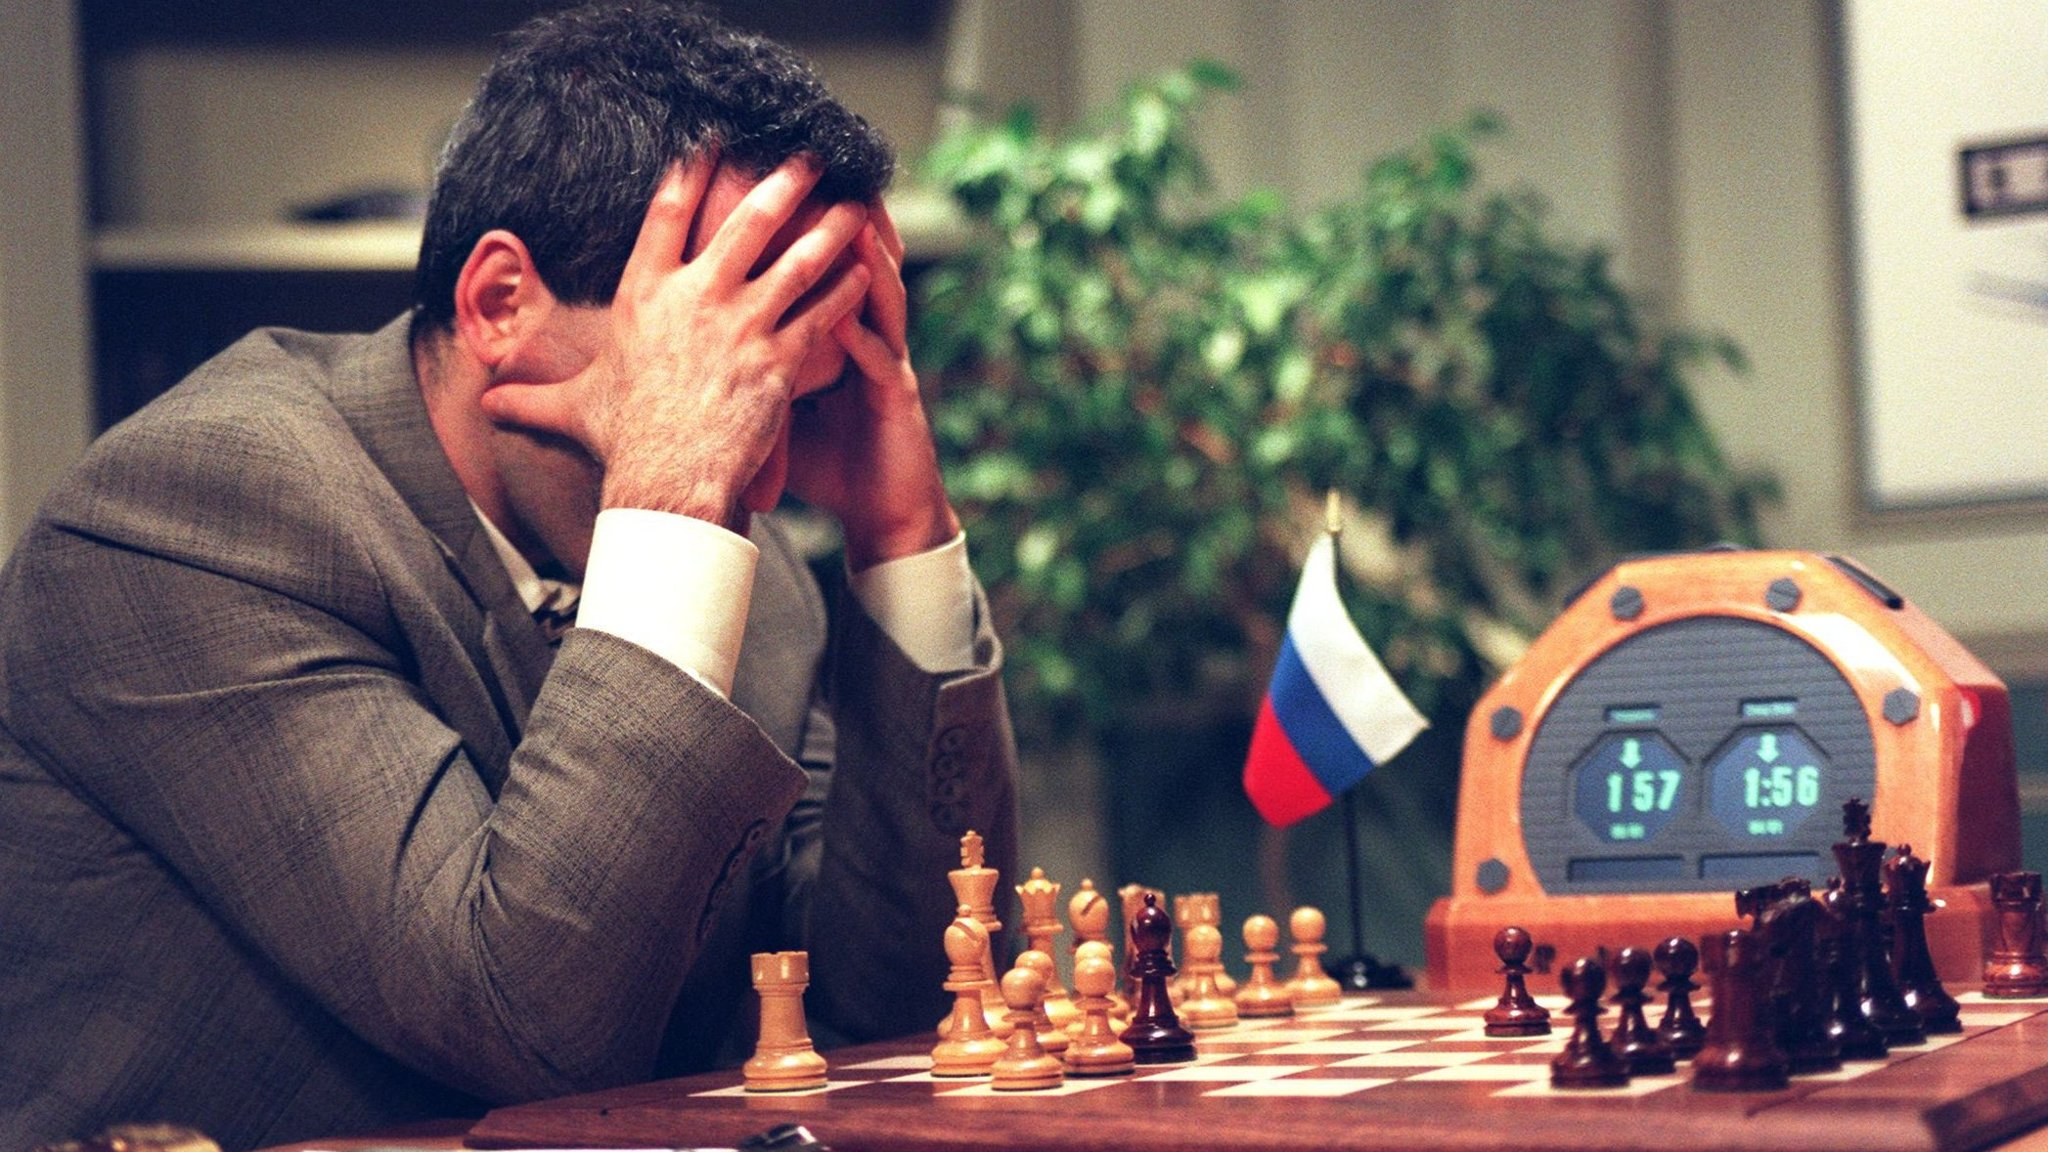
\includegraphics[width=0.4\textwidth]{kasparov}
				\includegraphics[width=0.4\textwidth]{CA}
				\caption{Kasparov vs Deep Blue e automato celular}
			\end{figure}
		\end{itemize}
	\end{frame}
	\section{Métodos de simulação}
		\subsection{Sistemas dinâmicos}
		\begin{frame}{O que é um sistema dinâmico?}
			\begin{itemize}[<+->]
				\item Em resumo, um \textbf{sistema dinâmico} é um sistema que varia no tempo;
				\item o sistema é descrito uma variavel que define o estado do sistema;
					\begin{equation}
						s(t)
					\end{equation}
				\item o estado pode ser um vetor (multivariavel);
					\begin{equation}
						s(t)=(s(t),...,s_n(t))^{T}
					\end{equation}
				\item e para adicionar a \emph{dinâmica} no sistema, é necessário definir como o \textbf{estado} varia no tempo.
				\item qual a forma mais convencional de fazer isso matematicamente?
				\begin{equation}
					\dot{s}(t) = \frac{s(t)}{dt} = f(s(t))
				\end{equation}
			\end{itemize}
		\end{frame}
		\begin{frame}{Representações de sistemas dinâmicos}
			\par Temos geralmente duas formas de representar o tempo em sistemas dinâmicos, e isso normalmente depende da dinâmica do sistema e como isso será definido.
			\begin{itemize}[<+->]
				\item \textbf{Tempo discreto:} os tempo nos sistemas dinâmicos são representados \textbf{relações recorrentes} tambem chamado de \textbf{equações de diferenças}.
				\begin{equation}
					s(t+\Delta t) = f(s(t))
				\end{equation}
				\item \textbf{Tempo continuo:} já nos sistemas contínuos são representados por \textbf{equações diferenciais}, ordinárias (ODE) ou parciais (PDE).
				\begin{equation}
					\dot{s} = \frac{ds(t)}{dt} = f(s(t))
				\end{equation}			
			\end{itemize}
		\end{frame}
		\begin{frame}{Exemplo: Crescimento Populacional}
			\begin{itemize}[<+->]
				\item Vamos abordar um problema onde aplicação onde o objeto é simular o \textbf{"crescimento"} de uma população em um dado sistema.
				\item podemos começar modelando esse sistema, definindo a variável estado do sistema, que no caso é a população $P(t)$.
				\item Considerando que sabemos o estado atual da população $P(0)=P_0$, temos um IVP.
				\item De forma bastante resumida, podemos falar que os unicos processos que influenciam o estado da população é a $M(t)$ e o nascimento $N(t)$.
				\item então podemos definir que:
					\begin{equation}
						\dot{P}= \frac{P(t)}{dt} = N(t)-M(t)
					\end{equation}
				\item Possiveis funções para modelar os nascimentos e mortes poderiam ser:
					\begin{equation}
						B(t)=r_bP(t)
					\end{equation}
					\begin{equation}
						B(t)=r_dP(t)
					\end{equation}
			\end{itemize}
		\end{frame}
		\begin{frame}{Exemplo: Crescimento Populacional}
			\begin{itemize}[<+->]
				\item Podemos simplificar esse problema da seguinte forma:
					\begin{equation}
						\dot{P}=rP(t) \text{ onde } r=rb-rd
					\end{equation}
				\item E, por ser um modelo \textbf{muito} simples, podemos resolve-lo analiticamente.
					\begin{equation}
						P(t)=P_0e^{rt}
					\end{equation}
			\end{itemize}
		\end{frame}
		\begin{frame}{Exemplo: Crescimento Populacional}
			\begin{columns}
				\begin{column}{0.5\textwidth}
					\begin{itemize}
						\item $r > 0$: crescimento exponencial
						\item $r < 0$: decaimento exponencial
						\item $r = 0$: população constante
					\end{itemize}
				\end{column}
				\begin{column}{.5\textwidth}
					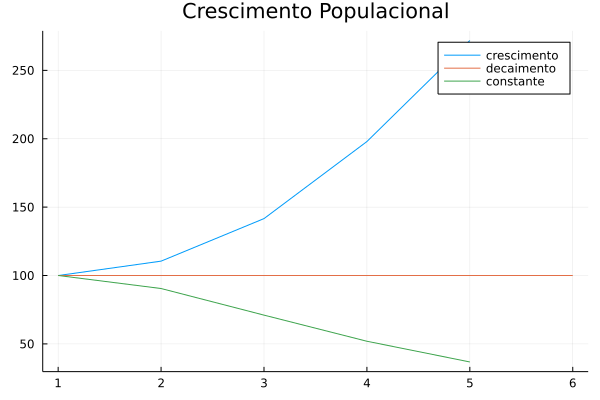
\includegraphics[width=\textwidth]{cres_pop}
				\end{column}
			\end{columns}
		\end{frame}
		\begin{frame}{Exemplo: Lotka-Volterra}
			\begin{itemize}[<+->]
				\item Expandindo a simulação aplicada a dinâmica populações, um modelo mais completo seria o modelo de \textbf{Lotka-Volterra}, tambem conhecido como \emph{presa-predador}.
				\item Suponha que você queira modelar as populações de gatos e ratos em uma ilha, com suas respectivas dinâmicas no tempos definidas pelas funções $g(t)$ em $r(t)$, respectivamente. Os gatos se alimentam de ratos e morrerão de fome sem eles.
				\item Portanto, qualquer equação diferencial que descreva a taxa de variação de $g(t)$ também deve envolver $r(t)$. Da mesma forma, a taxa de variação de $r(t)$ depende do número atual de $g(t)$.
			\end{itemize}
		\end{frame}
		\begin{frame}{Exemplo: Lotka-Volterra}
			\begin{itemize}[<+->]
				\item Isso apresenta algumas novas características do modelo para simulação, agora precisamos represetar dois \textbf{estados do sistema}, a população de gatos $g(t)$ e de ratos $r(t)$.
				\item Podemos modelar esse sistema como um \textbf{sistema de equações diferenciais}.
				\item E chegamos no \textbf{modelo de Lotka-Volterra}.
				\begin{equation}
					\frac{dr(t)}{dt}=\alpha r(t) - \beta r(t)g(t)
				\end{equation}
				\begin{equation}
					\frac{dg(t)}{dt}=\delta r(t)g(t) - \gamma g(t)
				\end{equation}
			\end{itemize}
		\end{frame}
		\begin{frame}{Exemplo: Lotka-Volterra (Solução)}
			\begin{columns}
				\begin{column}{0.5\textwidth}
					Parâmetros:
					\begin{itemize}[<+->]
						\item $\alpha$ : é a taxa de crescimento da população de ratos na ausencia de gatos. 
						\item $\beta$ : é a taxa de morte natural de gatos na ausencia de ratos.
						\item $\delta$ : é a taxa de mortalidade por encontro de gatos com ratos.
						\item $\gamma$ : é a "conversão" de ratos em gatos.
						\item 
						\begin{equation}
							\frac{dr(t)}{dt}=\alpha r(t) - \beta r(t)g(t)
						\end{equation}
						\begin{equation}
							\frac{dg(t)}{dt}=\delta r(t)g(t) - \gamma g(t)
						\end{equation}
					\end{itemize}

				\end{column}
				\begin{column}{0.5\textwidth}
					\begin{center}
						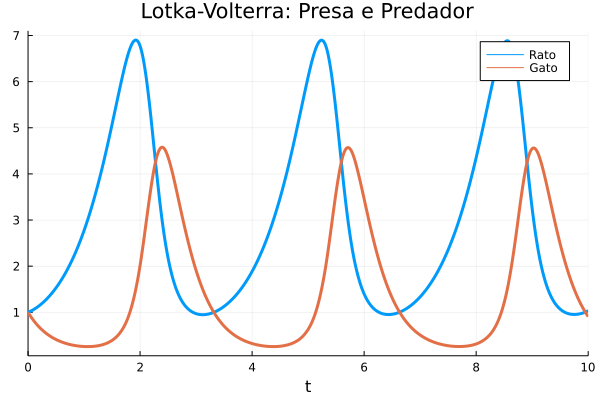
\includegraphics[width=\textwidth]{Lotka-volterra}
					\end{center}
				\end{column}
			\end{columns}
		\end{frame}
		\subsection{Monte Carlo}
		\begin{frame}{O que é metodo de Monte Carlo?}
			\begin{itemize}[<+->]
				\item O objetivo do metodo de monte de carlo é amostrar um processo estocástico e a partir disso, determinar propriedades estatísticas do fenomeno.
				\item no entanto, como é amostrado os eventos aleatórios?
				\item A principal sacada do metodo de Monte Carlo foi utlizar a função inversa de uma CDF (cumulative distribution function) para, a partir de um gerador de numeros aleatórios, definir o estado do evento gerado.
				\item Por exemplo, se jogarmos uma moeda 4 vezes, qual é a probabilidade de obtermos 3 caras e 1 coroa?
				\item podemos definir isso analiticamente pelo seguinte processo (distribuição binomial):
				\begin{equation}
					P(3 caras) = \binom{4}{3}\frac{1}{2}^2\big(1-\frac{1}{2})^1 = \frac{1}{4}
				\end{equation}
			\end{itemize}
		\end{frame}
		\begin{frame}{Simulação probabilidade Cara ou Coroa}
		\begin{center}
			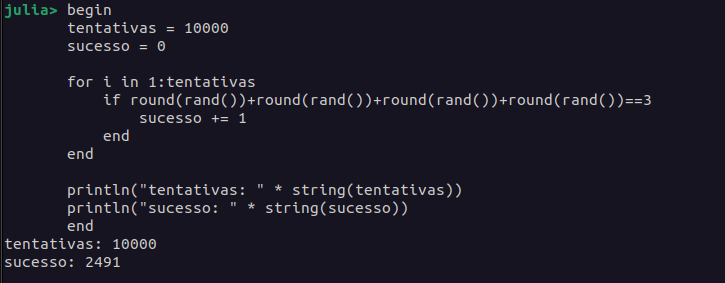
\includegraphics[width=\textwidth]{simul-monte-carlo}
		\end{center}
		\end{frame}
		\begin{frame}{Exemplo: Monte Carlo para análise de custo}
			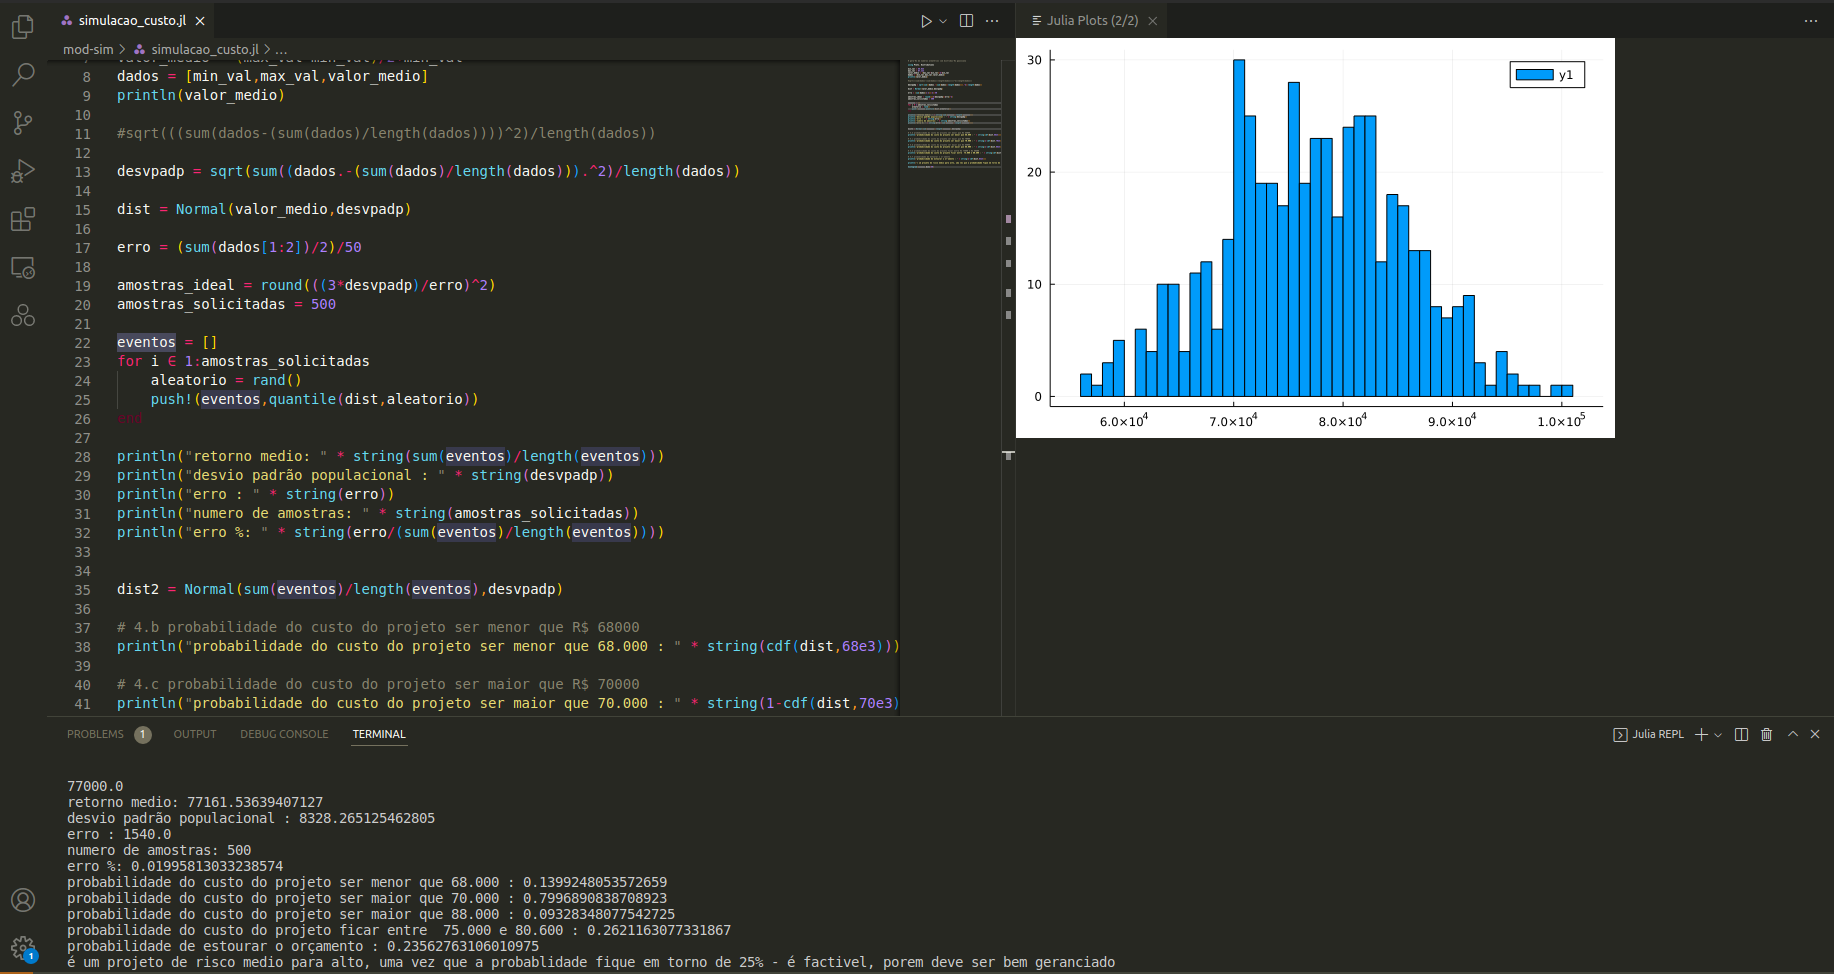
\includegraphics[width=\textwidth]{montecarlo2}
		\end{frame}
		\subsection{Automatos Celulares}
		\begin{frame}{Definição de Automatos Celulares}
			\begin{itemize}[<+->]
				\item Definindo a partir de um espaço discreto $\Omega$, um reticulado  de celulas de dimensões $n$.
				\item Realiza simulação em tempos discretos, calculado o \textbf{estado} de cada célula em cada passo no tempo $n$.
				\item Deve ser definido um conjunto discreto de estados $(S)$ possíveis por celula.
				\item Deve ser definido uma \textbf{regra de evolução $\Phi$} que define como ocorre a dinâmica do estado das células, na vizinhança $\mathcal{N}$
				\item a atualização do estado das celulas ocorre \textbf{paralelamente!}.
				\item Então para definir completamente um automato ceular precisamos da seguinte tupla:
				\begin{equation}
					<\Omega, S, \mathcal{N}, \Phi>
				\end{equation}
			\end{itemize}
		\end{frame}
		\begin{frame}{CA: Vizinhanças $\mathcal{N}$}
			\begin{columns}
				\begin{column}{0.5\textwidth}
					\begin{itemize}
						\item Vizinhança de Von Neumann;
						\item Vizinhança de Moore;
					\end{itemize}
				\end{column}
				\begin{column}{0.5\textwidth}
					\begin{figure}
						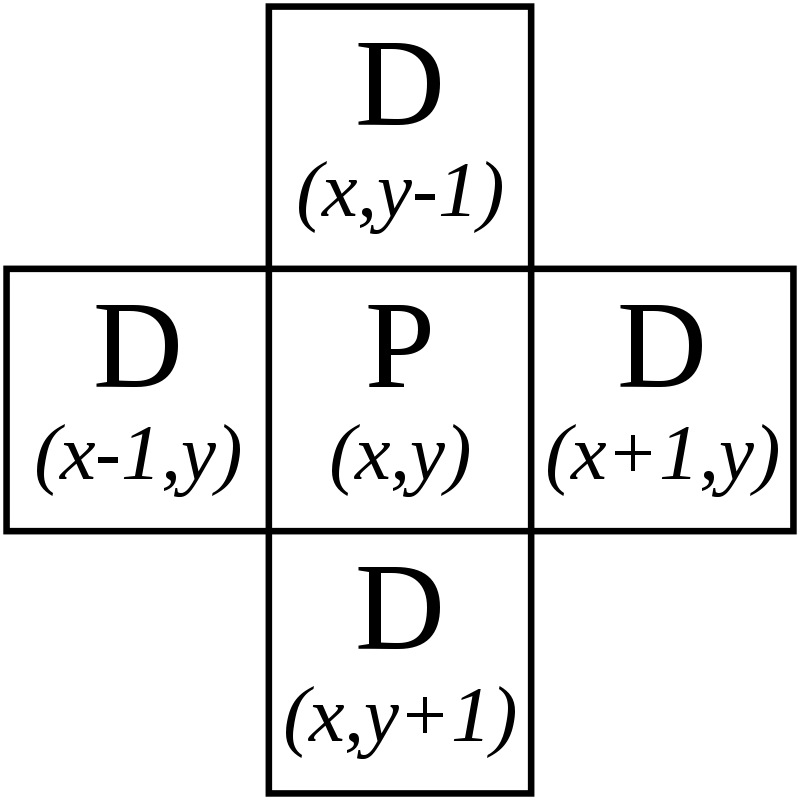
\includegraphics[width=0.3\textwidth]{neumann.png}
						\caption{Von Neumann $\mathcal{N}$}
					\end{figure}
				\begin{figure}
					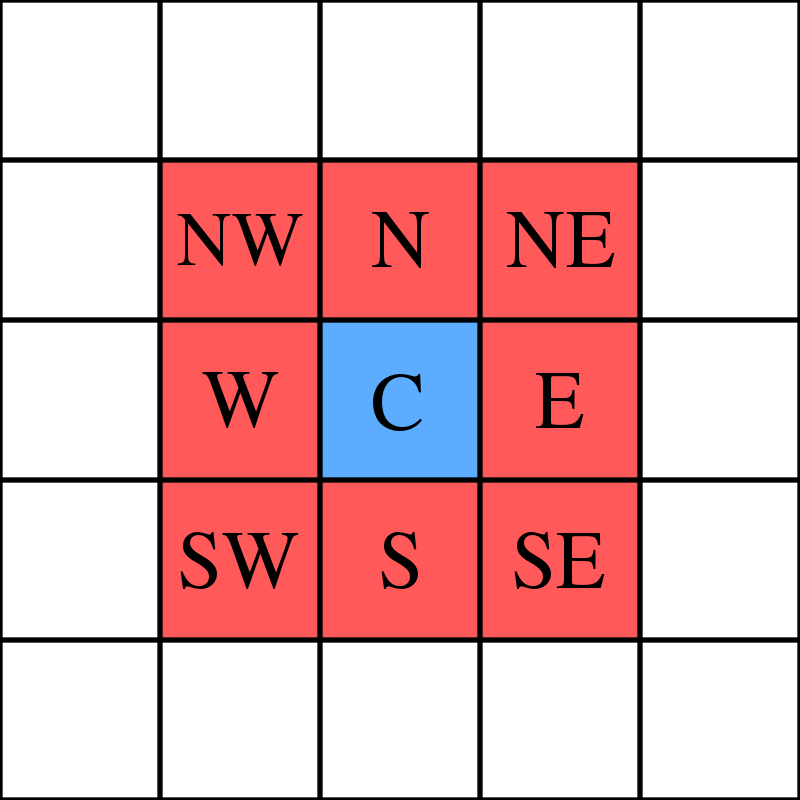
\includegraphics[width=0.3\textwidth]{moore.png}
					\caption{Moore $\mathcal{N}$}
				\end{figure}							
				\end{column}
			\end{columns}
		\end{frame}
		\begin{frame}{Exemplo: Jogo da Vida de Conway}
			\par Um exemplo classico de um automato celular é o \emph{Conway's game of life}, onde cada celula tem 2 estados, ou seja $S = <vivo, morto>$;
			\par O espaço $\Omega$ é um \textbf{reticulado infinito 2D}.
			\par Poder ser aplicado tanto em Neumann $\mathcal{N}$ ou Moore $\mathcal{N}$.
			\par e a regra de evolução $\Phi$ é definda por:
			\begin{itemize}
				\item qualquer célula com menos de 2 vizinhos vivos \textbf{morre} (subpopulação);
				\item qualquer célula com 2 ou mais vizinho vivos \textbf{vive} na proxima geração;
				\item qualquer célula viva com mais de 3 vizinhos vivos \textbf{morre} (sobrepopulação);
				\item qualquer célula morta com exatamente 3 vizinhos vira uma célula \textbf{viva} (reprodução);
			\end{itemize}
		\end{frame}
		\begin{frame}
			\par GIF do jogo da vida...
		\end{frame}
		\subsection{Simulação de eventos discretos}
		\begin{frame}{Simulação de Eventos Discretos}
			\begin{itemize}[<+->]
				\item Contrasta com simulações \emph{time-driven};
				\item Deve existir \textbf{eventos no tempo} que causam alterações significantes no comportamento do sistema;
				\item O sistema é simulado por \textbf{saltos entre eventos} no tempo.
			\end{itemize}
		\end{frame}
		\begin{frame}{Requisitos para executar uma DES}
				\begin{itemize}[<+->]
					\item deve ser possivel \textbf{calcular analiticamente} o estado do sistema, em qualquer valor no tempo, entre dois eventos.
					\item Os eventos devem ocorrer em uma posição no tempo $t \in \mathbb{R}^{+}$.
					\item Apenas 1 evento pode ocorrer de cada vez.
				\end{itemize}
		\end{frame}
		\begin{frame}{Descrição de uma simulação por eventos discretos}
			\begin{itemize}[<+->]
				\item O sistema é composto de varias entidades $i$, que representam os \emph{passos} da simulação.
				\item Cada passo é descrito pelo seu conjunto de estados $(s_i(t))$.
				\item Onde $S(t)$ é o conjunto $\{s_i(t)\}$ no instante de
				 tempo $t$.
			\end{itemize}
		\end{frame}	
		\begin{frame}{Descrição dos eventos}
			\begin{itemize}[<+->]
				\item Cada evento $j$ é associado com uma ação $a_j$.
				\item Cada ação $a_j$ muda o estado do sistema:
				\begin{equation}
					a_j: S(t_i) \rightarrow S(t_{i+1})
				\end{equation}
				\item O evento é a \textbf{causa}, a ação é o \textbf{efeito}.
			\end{itemize}
		\end{frame}
		\subsection{Elementos Finitos}
		\begin{frame}{Método dos elementos finitos}
			\begin{columns}
				\begin{column}{0.5\textwidth}
						\begin{itemize}[<+->]
						\item Embora o método dos elementos finitos seja um metodo númerico para solução de PDE, ele é amplamente utilizado para simulação fenômenos físicos na fisica e na engenharia.
						\item A principal vantagem do metodo dos elementos finitos é a possibilidade de solução númerica para PDEs que descrevem a dinâmica espaco-temporal em geometrias complexas. problemas que dificilmente possuem solução analitica.
						\end{itemize}
				\end{column}
				\begin{column}{0.5\textwidth}
					\begin{figure}
						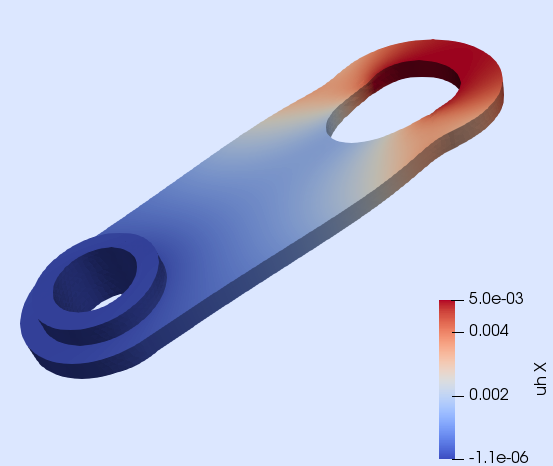
\includegraphics[width=0.5\linewidth]{fe1}
						\caption{Elasticidade Linear}
						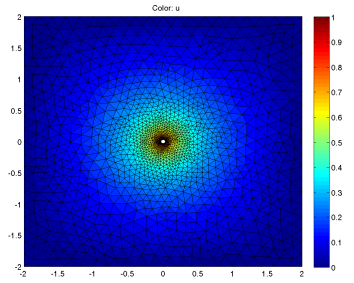
\includegraphics[width=0.5\linewidth]{fe2}
						\caption{Campo Elétrico}				
					\end{figure}
				\end{column}
			\end{columns}
		\end{frame}
		\begin{frame}{Metodo dos Elementos Finitos}
			\begin{itemize}
				\item O \textbf{metodo dos elementos finitos} consiste na criação de uma \textbf{malha} que representa a geometria do espaço onde o campo escalar ou vetorial ocorre. esse passo é conhecido como \textbf{discretização do domínio} é comum para metodos númericos.
				\item O proximo passo é aproximação da solução por uma \textbf{interpolação polinomial} em cada elemento.
				\item Definição de matrizez compostas das \textbf{interpolações polinomiais} para representar o sistema global para o dominio de solução.
				\item Aplicar algoritmo de solução do sistema global. (variais opções disponiveis), mas normalmente é utilizado livrarias de algebra linear de \textbf{HPC} como \textbf{LAPACK} e \textbf{BLAS}.
			\end{itemize}
		\end{frame}
		\begin{frame}{Exemplos: Elementos finitos}
			\begin{columns}
				\begin{column}{.5\linewidth}
					\begin{figure}
						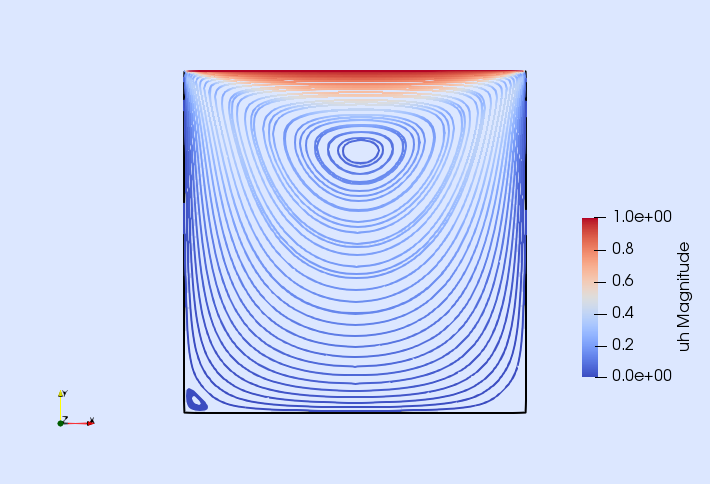
\includegraphics[width=\linewidth]{navierstokes2d}
						\caption{Navier-stokes para fluídos imcompressíveis}
					\end{figure}
				\end{column}
				\begin{column}{.5\linewidth}
					\begin{figure}
						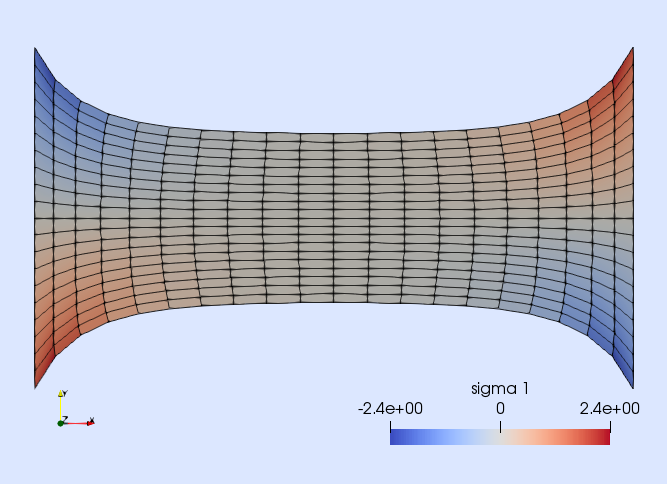
\includegraphics[width=\linewidth]{neohook}
						\caption{Deformação de material hiperelástico}
					\end{figure}
				\end{column}			
			\end{columns}
		\end{frame}
		\begin{frame}{Referências}
			\fontsize{9pt}{10pt}
			\textbf{Referências:}
			\bibliographystyle{abbrv}
			\bibliography{metsim.bib}
		\end{frame}
\end{document}
